\documentclass[11pt]{article}

%defines page size and margins
\usepackage{geometry}
\geometry{
    letterpaper,
    left=1in,
    right=1in,
    top=1in,
    bottom=1in,
}

%Sets spacing for entire document
\usepackage{setspace}
\singlespacing

%Package for reducing space in between list items
\usepackage{enumitem}

%Line break inbetween each paragraph
\usepackage[parfill]{parskip}

%Math symbols
\usepackage{gensymb}

%dope tables
\usepackage{array}
\usepackage{float}

%Image path
\usepackage{graphicx}
\graphicspath{ {../Images/} }

%Makes lists easier
\newcommand{\ol}[1]{\begin{enumerate}[noitemsep, topsep=0pt]#1\end{enumerate}}
\newcommand{\ul}[1]{\begin{itemize}[noitemsep, topsep=0pt]#1\end{itemize}}
\newcommand{\li}[1]{\item#1}

\begin{document}

{\large\noindent 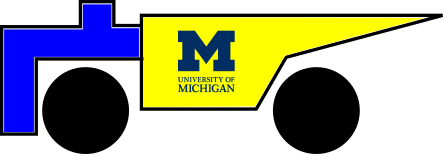
\includegraphics{Logo}[H]

\noindent Tonka

\noindent Rishabh Shah

\noindent October 2, 2017}

\section*{Transmission}
\begin{table}[H]
	\centering
	\begin{tabular}{|r|c|c|}
		\hline
		\textbf{Gear} & \textbf{Diameter (inch)} & \textbf{Number of teeth} \\
		\hline
		One & 5 & 28 \\
		\hline
		Two & 7 & 38 \\
		\hline
		Three & 9 & 48 \\
		\hline
	\end{tabular}
	\caption{Front gear assembly specifications}
\end{table}
\begin{table}[H]
	\centering
	\begin{tabular}{|r|c|c|}
		\hline
		\textbf{Gear} & \textbf{Diameter (inch)} & \textbf{Number of teeth} \\
		\hline
		One & 4 & 28 \\
		\hline
		Two & \(3\frac{1}{2}\) & 24 \\
		\hline
		Three & \(3\frac{1}{4}\) & 21 \\
		\hline
		Four & 3 & 18 \\
		\hline
		Five & \(2\frac{3}{4}\) & 16 \\
		\hline
		Six & \(2\frac{1}{4}\) & 14 \\
		\hline
	\end{tabular}
	\caption{Rear gear assembly specifications}
\end{table}
\begin{table}[H]
	\centering
	\begin{tabular}{|r|c|c|}
		\hline
		\textbf{Gear} & \textbf{Diameter (inch)} & \textbf{Number of teeth} \\
		\hline
		Upper & \(1\frac{3}{4}\) & 11 \\
		\hline
		Lower & \(1\frac{3}{4}\) & 11 \\
		\hline
	\end{tabular}
	\caption{Derailleur gear assembly specifications}
\end{table}

\section*{Linkages}

\section*{Bearings}

\end{document}